\documentclass{beamer}          %幻灯片宏包
\usepackage{beamerthemesplit}   %主题风格
%\usetheme{Hannover}   %主题风格
\usepackage{graphics}
\usepackage{CJKutf8}            %支持中文
\begin{document}
\begin{CJK*}{UTF8}{}            %中文支持
  \CJKfamily{gbsn}              %字体
\title{自由思想 \ 开源力量}     %添加标题
\subtitle{GNU/Linux}           %附标题
\author{Li \ Junpeng}           %添加作者
\institute{
Communications Technology of Information Engineering\\
  Liuzhou Railway Professional Technology College 
}
\date{\today{}}                 %添加日期

\frame{\titlepage{}}            %添加主题幻灯片

\frame{\frametitle{讨论内容概述}
\pause{}
\begin{itemize}
\item 介绍linux,人物,作用,嵌入式
\item 介绍GNU计划
\item 介绍为什么使用linux
\end{itemize}
}

\frame{\frametitle{What's Linux?}
 \begin{figure}                 %图片
       \begin{center}
       
\includegraphics[width=1cm, height=1cm]{logo_linux.jpg}
       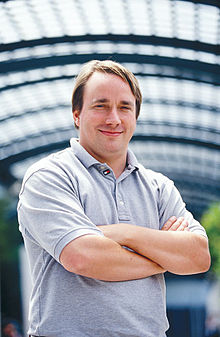
\includegraphics[width=2cm, height=2.5cm]{Linus_Torvalds.jpeg}
       \end{center}
\end{figure}
\pause{}
\begin{itemize}
  \item 什么是Linux? \\
\pause{} 
\ \ http://zh.wikipedia.org/zh-cn/Linux \\ %介绍人物
 \pause{}
系统 \ - \pause{}核心 \ - \pause{} GNU/Linux \ - \pause{} 发行版 \\
\pause{}
\item Linux优势? \pause{}\\
自由,免费,开源,工具丰富,手机(Android),有趣流行,很多另人兴奋的技巧,资源开销底,灵活,个性化,社区活跃 \\ \pause{}
高校科研教学,原生体编程环境,嵌入式,服务器,群集,无穷无尽的学习动力,思想超前不再受限于windows
\end{itemize}
}

\frame{\frametitle{What's Linux?}
 \begin{figure}                 %图片
       \begin{center}
       
\includegraphics[width=1cm, height=1cm]{logo_linux.jpg}
       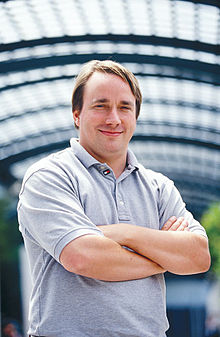
\includegraphics[width=2cm, height=2.5cm]{Linus_Torvalds.jpeg}
       \end{center}
\end{figure}
       \begin{itemize}

\item Linux很强大?\\
真正用了才知道....\pause{} 超级计算机,工作站,多用户,协作,给有的印象是,什么都能做,特别是高科技 
\pause{}
\item linux 很难学? \\
兴趣、搜索引擎是最好的老师。\\ \pause{}
另一途径,多上机操作,不懂先找找man \\ \pause{}
懂用vi , ls , cd , cp , mv , man 就算入门\\ \pause{}
开源社区乐于助人帮助他人,你我他共同学习\\\pause{}
Linux经典的书籍丰富,电子书免费 \\\pause{}
寻找共同语言 \  IRC 交流
       \end{itemize}
}
\frame{                        %一个frame,即一张幻灯片
  \frametitle{伟大的GNU计划} %此幻灯片标题
 \begin{figure}                 %图片
       \begin{center}
         
\includegraphics[width=1.5cm, height=1.5cm]{logo_heckert_gnu_left.jpg}
         
\includegraphics[width=2.5cm, height=2cm]{Richard_Stallman.jpeg}%介绍人物
       \end{center}
\end{figure}
%  \tableofcontents{}            %目录
\begin{itemize}
  \item 什么是GNU?\pause{}
    http://zh.wikipedia.org/zh-cn/GNU \pause{} \\
  GNU项目 \ - \pause{} GNU授权协议 \ - \pause{} 自由软件 \ - \pause{} 神器Emacs \pause{}\\ 
GNU =  GNU IS NOT UNIX \ ! \pause{}
\item 什么是GNU/Linux \pause{} \\
http://zh.wikipedia.org/zh/GNU/Linux \\ \pause{}
发行版 \ - \pause{} 国内发行版 \ - \pause{} 自己的发行版本\pause{} \\
\end{itemize}
}

\frame{\frametitle{基本命令操作}
Linux强大的生命力在于其高效的字符命令行界面 \pause{}
  \begin{itemize}
    \item 登录 \ - 输入系统管理员分配的用户名,密码
\item 登出 \ - logout
\item 列表 \ - ls 
\item 切换目录 \ - cd
\item 复制文件 \ - cp
\item 移动或重命令 \ - mv
\item 帮助 \ - man
\item 查找 \ - find
  \end{itemize}
}

\frame{\frametitle{有趣的演示}
演示一些有趣的工具,详细介绍命令的特征 \pause{}

\begin{itemize}
  \item sl \pause{} \\
    sl -alef \\ apt-get source sl
\item typespeed
\item vi
\item emacs
\item tmux
\end{itemize}

}
\frame{\frametitle{熟悉必要工具}
 \begin{itemize}
  \item<1-> emacs \ \   
\includegraphics[width=0.5cm, height=0.5cm]{emacs23.jpg}
  \item<2-> vi/vim  \  
\includegraphics[width=0.5cm, height=0.5cm]{Vimlogo.png}
  \item<3-> tmux
  \item<4-> find
  \item<5-> gcc
  \end{itemize}
}
\end{CJK*} 
\end{document}
